Carabineros, Chile's national police force, was founded in 1927. Through most of our study period, Carabineros operated under the Ministry of Defense, which oversaw both military and police functions until domestic security responsibilities were transferred to the Ministry of Interior in 2011.\footnote{Currently, Carabineros reports to the Ministry of Public Security, created in 2024 to focus exclusively on domestic security.}

Carabineros' mission, functions, and structure are established by Law 18.961 and the Regulation on Carabineros' Organization (Reglamento de Carabineros) \citep{Ley18961,ReglamentoCarabineros1989}. Under this framework, Carabineros is a professional, disciplined, and hierarchical police institution whose mission is to preserve public order and security with a central emphasis on preventive policing. The General Director heads the strategic level, responsible for defining doctrine and institutional strategy, while the Subdirector coordinates implementation. The Directorate of Order and Security administers police functions at the tactical level.

Territorially, Carabineros is organized into zones that oversee \emph{prefecturas}. Zones and \emph{prefecturas} are primarily management layers. Zones map roughly one-to-one to Chile's regional divisions, with two exceptions: the Metropolitan Region of Santiago---the most populated in the country---and La Araucanía---which has recently experienced significant social conflict---are each divided into two zones. Each zone is subdivided into \emph{prefecturas}---54 nationwide---which supervise 227 \emph{comisar\'ias}, the main operational units at the tactical level. These \emph{comisar\'ias} oversee smaller units---\emph{subcomisar\'ias}, \emph{tenencias}, \emph{retenes}, \emph{puestos}, and \emph{avanzadas}---that operate within their assigned jurisdictions.\todo{JORGE: Since we need to cut on the manuscript, I believe this paragraph is a good candidate to be removed or shortened.}

In practice, the \emph{comisar\'ia} is the basic unit of routine frontline policing and, in most municipalities, serves as the territorial anchor of police work. Officers conduct patrol, surveillance, prevention, and first response at this level. In most municipalities, a single \emph{comisar\'ia} covers the entire municipal territory, though larger municipalities may have multiple ones. Santiago, for instance, has four. %By contrast, 112 municipalities---mostly remote or rural---have no \emph{comisar\'ia} and are served through smaller subordinate posts linked to a \emph{comisar\'ia}. 
All municipalities that adopted \emph{Plan Cuadrante} during our study period had a \emph{comisar\'ia}. With the exception of 9 municipalities, each had a single \emph{comisar\'ia} covering the full municipal territory. On average, a \emph{comisar\'ia} in our sample covered 1,608 square kilometers and served 57,642 inhabitants. %Of these, 17 had no subordinate units, whereas the remaining 79 had between one and nine.

\emph{Plan Cuadrante} was introduced within this institutional framework without altering Carabineros' hierarchical structure or its strategic and tactical levels. The reform emerged in a context of rising victimization and insecurity, with the explicit goal of reversing these trends \citep{PCSP2014}. Its central innovation was a shift toward a beat policing model. In the criminology literature, beat policing refers to assigning officers to fixed territorial areas so they can accumulate local knowledge, strengthen ties with residents, and respond more effectively to local crime patterns \citep{cordner1995community,skogan1997comminuty}. In practice, the catchment area of police forces in municipalities adopting \emph{Plan Cuadrante} was partitioned into smaller, fixed geographic units (quadrants), to which officers were permanently assigned. Rather than building new infrastructure, the reform redefined the territorial responsibility of officers in already existing police stations \citep{DIPRES2007_largo}.\footnote{In 2016, Carabineros launched the \emph{Plan Cuadrante 2.0} program in those municipalities served by \emph{Plan Cuadrante}. While this reform introduced additional reforms aimed at integrating the community into the provision of security and building capacity to gather and analyze crime data in police stations, this paper's study period ends before these improvements were introduced.} This represented a clear break from the pre-reform system, in which officers rotated across broad operational territories, very often spanning entire municipalities.

Carabineros began piloting \emph{Plan Cuadrante} in 1998. The program expanded gradually through 2013, as shown in Panel (a) of Figure \ref{fig:figure01}, reaching 150 urban municipalities and covering roughly 90\% of Chile's population.\footnote{Further details about the expansion of \emph{Plan Cuadrante} are provided in Online Appendix \ref{sec:appendixA} and Table \ref{tab:implementation}.} Online Appendix A provides further details about the rollout of the program. The rollout was designed to follow a municipality ranking based on a weighted index of victimization, police resource deficits, drug prevalence, unemployment, and demand for police services, with annual entry determined by available budget.\footnote{The weights assigned to each component changed on a yearly basis \citep{DIPRES2007_largo,DIPRES2014}.} In practice, however, Budget Office evaluations show that adoption diverged from this ranking for undocumented reasons, so the rule operated more as a loose guideline than as a binding assignment mechanism \citep{DIPRES2014}.

\FloatBarrier
%--- Implementation
\begin{figure}[h!]
    \centering
    \caption{Implementation of \emph{Plan Cuadrante}}
    \label{fig:figure01}
    \begin{subfigure}{0.58\textwidth}
        \centering
        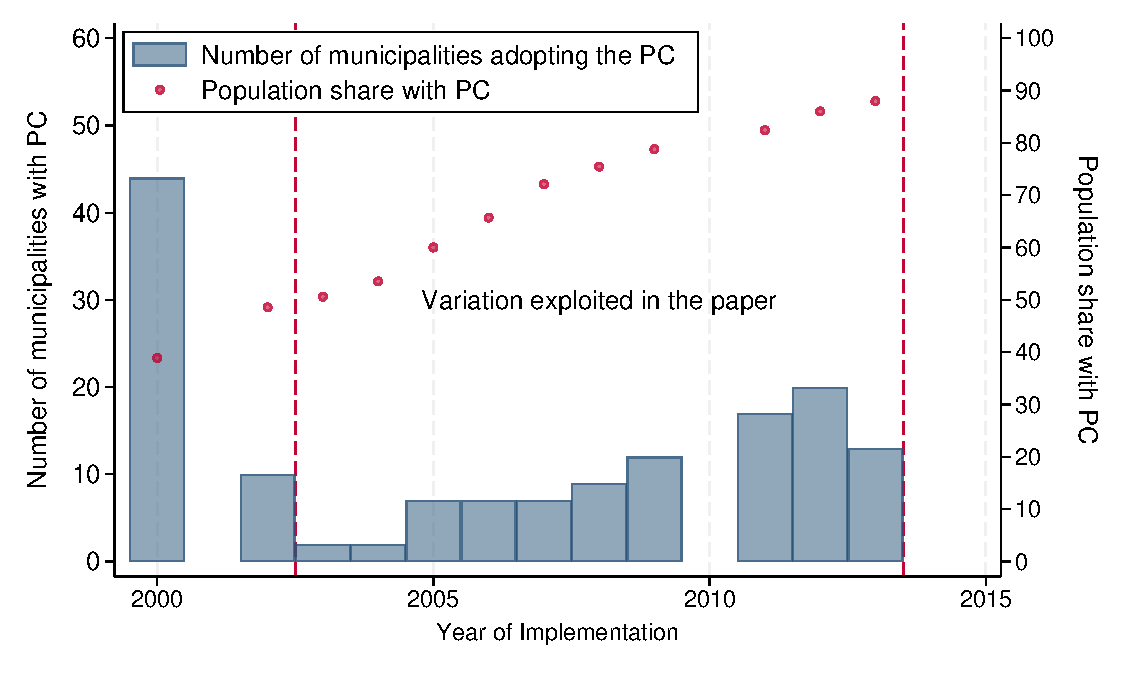
\includegraphics[width=1\textwidth]{../manuscript/Graphs/Graph_PCvariation.pdf}
        \caption{Adoption of \emph{Plan Cuadrante}}
    \end{subfigure}
    \\
    \begin{subfigure}{\textwidth}
    \centering
    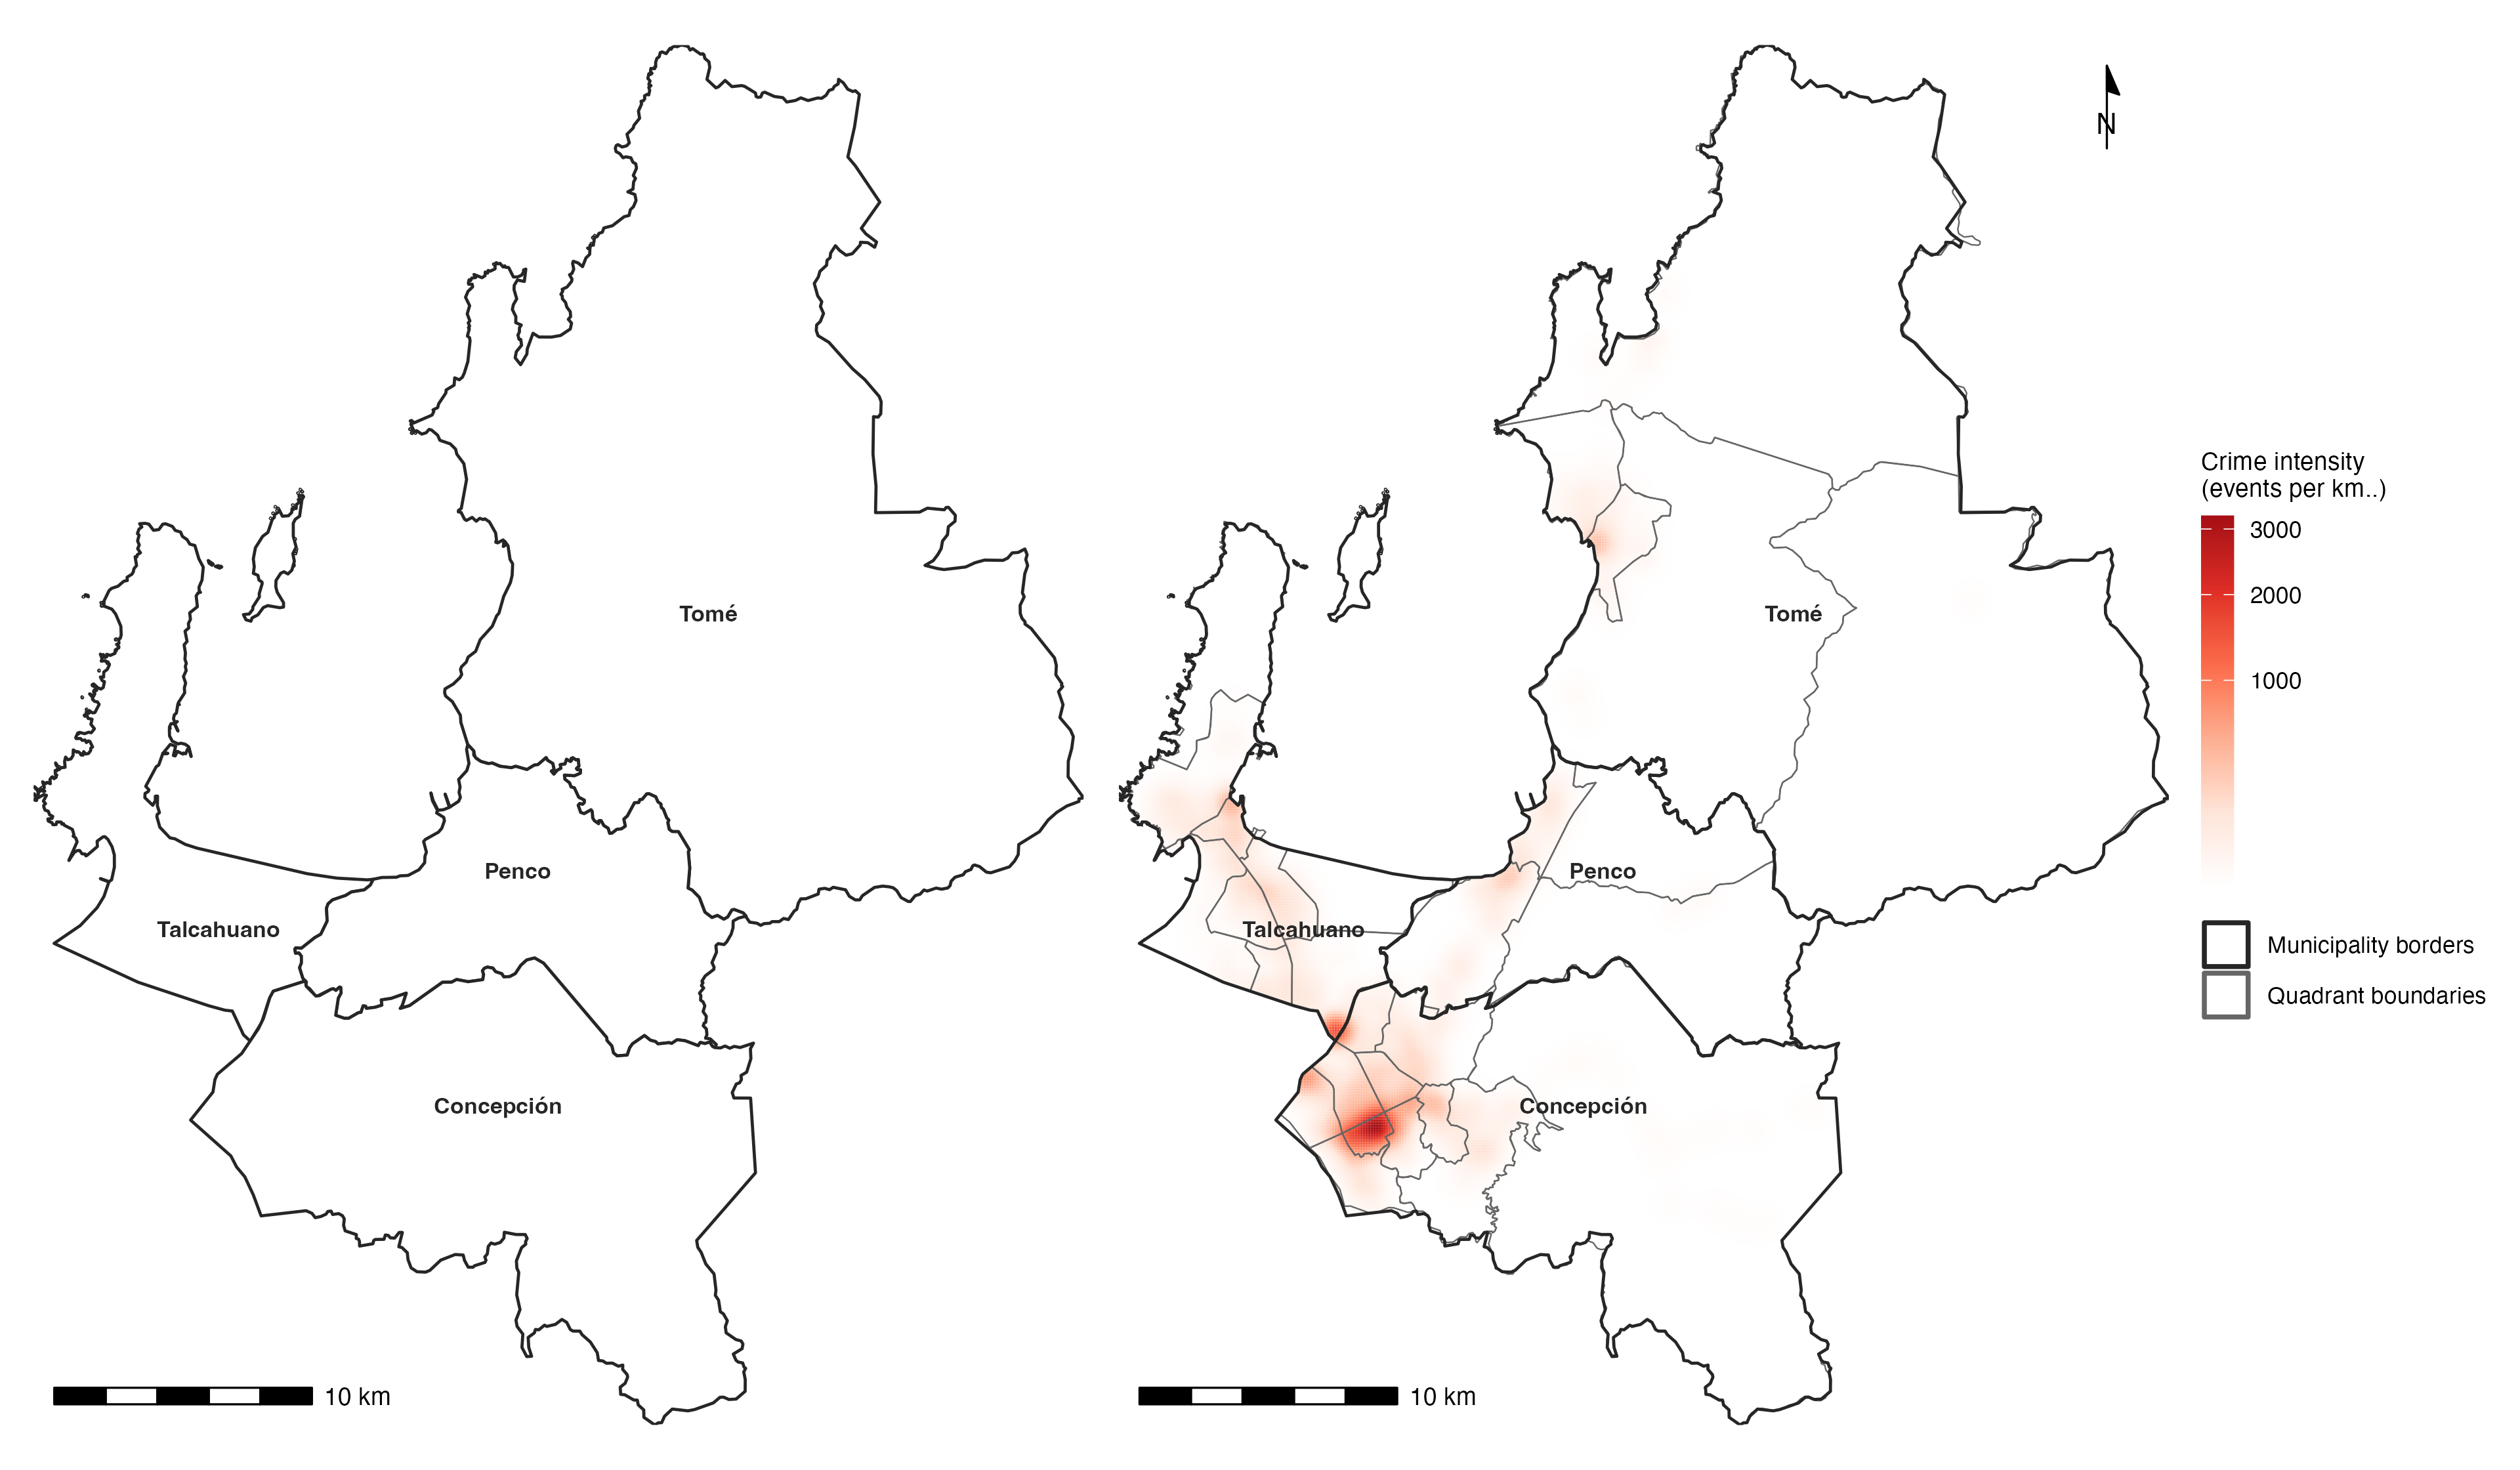
\includegraphics[width=0.65\linewidth]{../manuscript/Graphs/Graph_PCexample_combined.png}
    \caption{\emph{Plan Cuadrante} in the Concepci\'on area}
    \end{subfigure}%
 %   \\
 %   \begin{subfigure}{0.58\textwidth}
 %       \centering
 %       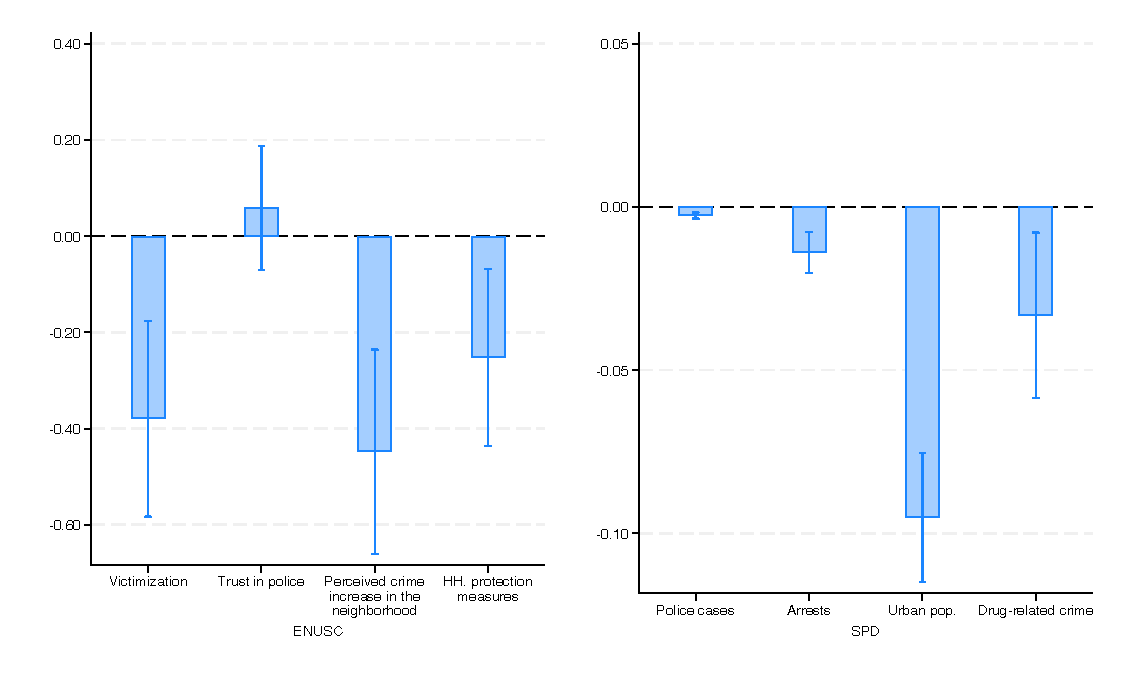
\includegraphics[width=1.1\textwidth]{../manuscript/Graphs/results_predictorsPC_combined.pdf}
 %       \caption{Time of Adoption and Municipality Characteristics}
  %  \end{subfigure}%
    \\[12pt]
    \begin{minipage}{0.95\textwidth}
    \footnotesize Notes: Panel (a) shows the number of municipalities adopting the \emph{Plan Cuadrante} each year (bars), while the circles above them illustrate the cumulative share of the Chilean population living in a municipality with the \emph{Plan Cuadrante} already in place. Panel (b) depicts the metropolitan area of Concepci\'on, the second-largest in Chile: the left map shows its four municipalities---the original police catchment areas---and the right map overlays the Carabineros quadrants together with a kernel-density estimate of all types of robberies and thefts recorded by the police (both reported crimes and arrests). It illustrates how \emph{Plan Cuadrante} subdivided each catchment area (which corresponds to the territory of a municipality) into smaller quadrants, as well as the spatial concentration of crime within them.
    \end{minipage}
\end{figure}
\clearpage

\FloatBarrier

Conceptually, police effectiveness can be viewed as a function of three inputs: total resources, territorial deployment, and policing strategy. Although in some municipalities police resources were increased significantly to operationalize the beat policing model \citep{DIPRES2007_largo,DIPRES2014}, the program primarily transformed the latter two elements. The creation of quadrants was accompanied by permanent geographic assignment of officers to specific areas. This change was operationally critical. By making officers responsible for their quadrant, it encouraged accumulation of local knowledge and stronger community ties, allowing them to adapt patrols and prevention activities to local crime patterns. Importantly, this was not driven by program-specific operational directive changes. Throughout the period we study, a single national set of operational guidelines applied to officers in both treated and control municipalities \citep{Manual_Carabineros2018,DIPRES2007_largo}. Thus, while the average effects we document on crime and crime perception likely reflect combined changes in the three elements we discuss---i.e., resources, deployment, and strategy---the deployment change itself was essential to operationalizing the reform. We discuss the drivers of the effects we document in Section \ref{mechanisms}.

Quadrant size and shape were determined by local police authorities based on factors such as road networks, geographic features, and available resources. In principle, resource allocation across quadrants followed demand for police services, measured in Equivalent Surveillance Units (UVEs); in practice, the station commander retained discretionary authority, as was also the case prior to \emph{Plan Cuadrante} \citep{DIPRES2014}. Municipalities implementing \emph{Plan Cuadrante} were subdivided into an average of seven quadrants, each typically staffed by approximately three officers per shift. On average, each quadrant covered 185 square kilometers and served 13,466 inhabitants. Panel (b) of Figure \ref{fig:figure01} illustrates this structure, showing the 29 quadrants created across the four municipalities of the Concepción metropolitan region---Chile's second-largest metropolitan area and the largest in our sample. Quadrants represented approximately 14\% of the original \emph{comisar\'ia} territory. Officers continued to operate from the same police station but were permanently assigned to a specific sub-area within its jurisdiction. While Carabineros' hierarchical structure limits frontline officer decision-making authority, each quadrant was assigned a Quadrant Delegate (\textit{Delegado de Cuadrante}), a non-commissioned officer, responsible for immediate operational decisions within the quadrant.

\emph{Plan Cuadrante} may affect public safety through two complementary channels: deterrence and police effectiveness, understood as the capacity to respond to and resolve crimes. The changes induced by \emph{Plan Cuadrante}---permanently assigning officers to well-defined neighborhoods and, in some municipalities, increasing available resources---can increase both police visibility and local knowledge. As officers repeatedly patrol the same area, they become familiar with its streets, residents, and routines, which can raise the perceived probability of identification and apprehension and reduce the expected returns to crime. At the same time, this deeper knowledge of local territory and communities can improve police response and case resolution once crimes occur. The reform therefore likely affects both dimensions. Consistent with this interpretation, in Section \ref{results} we document declines in victimization and in reported crime---patterns consistent with deterrence---together with increases in arrests, consistent with improved police effectiveness.

Although beat policing shares features with other policing approaches, such as hot-spot policing and community-based policing, which have been widely studied, it has distinctive features that make it worth studying as an independent approach. Hot-spot policing concentrates resources in high-crime areas and does not focus on building local knowledge and community ties. It is typically implemented through targeted interventions at specific locations rather than systematic territorial organization, and the same officers are not necessarily sent repeatedly to the same areas. Evidence on hot-spot policing is mixed, with some studies showing crime reductions in targeted areas but also potential displacement effects \citep{SR_1}. \emph{Plan Cuadrante}, by contrast, subdivided all urban municipalities into quadrants with permanent officer assignment. As Panel (b) of Figure \ref{fig:figure01} illustrates, some quadrants contained crime hot-spots, but many did not. The reform thus addressed entire urban territories rather than specific high-crime areas, potentially mitigating displacement effects associated with hot-spot policing.

Community-based policing emphasizes building relationships with residents and addressing underlying social issues, and typically involves active community participation in defining strategy and priorities---in some cases, even assuming surveillance and prevention responsibilities. While increasing trust in the police and strengthening community ties were among the declared goals of \emph{Plan Cuadrante}, and may have resulted from its territorial reorganization, the community was not formally involved in the provision of security.\footnote{The \emph{Plan Cuadrante}'s original design contemplated a formal community integration model (MICC) with a Community Affairs Office (\textit{Oficina de Asuntos Comunitarios}) and a dedicated officer in each police station. However, this model was not implemented during our study period. Independent program evaluations from the Budget Office document that these Community Affairs Offices did not exist and had no dedicated personnel, budget, or structured activities in the period we study \citep{DIPRES2007_largo,DIPRES2014}. The community integration model was piloted in four police stations during 2012--2013, none of which are in our analytical sample. Financing was then discontinued in early 2014 and only restored and expanded after our study period ends.}%
 %Similarly, Operations Offices (\textit{Oficina de Operaciones}) formally assigned crime analysis functions but relied on paper-based entry systems, lacking digital infrastructure, analysts, or centralized data systems throughout the study period \citep{DIPRES2014}. Both the community integration model and crime analysis function were substantively implemented only with \emph{Plan Cuadrante} 2.0 (2015--2017) \citep{Carabineros2018}, outside our study period.}

In recent decades, police departments worldwide have transitioned toward beat policing reforms \citep{NASEM2018,PCSP2014}, yet the effectiveness of this model has not been rigorously assessed. Although the beat policing approach introduced through \emph{Plan Cuadrante} shares features with programs previously studied in the economic literature, its distinctive characteristics---comprehensive territorial reorganization and systematic local officer specialization---make it a valuable case for studying how deployment and policing strategies not yet examined in the economics literature affect crime and crime perception.

